
\subsection{Autonomous Operations}
\label{sec:autonomous}

To ensure the system is aligned with CASA regulations in accordance with Objective 2, the system will maintain constant communication with a ground based operator. The autonomous operations capability will extend to the detection of a suitable landing location and the descent of the UAV.

\subsubsection{Theory}

Based on reviewed literature, systems that use cameras to perceive the surrounding environment commonly use Python and OpenCV to perform image analysis. As described by \citeauthor{Tom5} (\citeyear{Tom5}), the three processes required for successful landing pad detection and landing are detection, tracking and displacement vector calculation. These processes will be performed by adapting existing algorithms to meet the specific needs of the application and implementing it on a micro-controller.




\subsubsection{Method}

The development of the system capable of landing site detection will be done in phases of increasing complexity.\\

An initial review of existing image segmentation algorithms will result in a system capable of simple colour and pattern detection. This can be implemented independently from the UAV and will serve as a proof of concept. Once developed, the software can be implemented using the onboard hardware.\\

Increasing the complexity of the recognition strategy will allow for more detailed perception of the environment and increase the reliability of future autonomous capabilities. As detailed in literature, it is important that the landing target can be detected and used to orient the drone when only partially visible and at varying distances. This will require the landing target detection algorithm to detect more complex shapes, and be based on more than basic colour detection.\\

% This development will verify the functionality of the 


This system will then be used as a base in which to implement and test a autonomous guidance system, ultimately capable of providing input commands to the onboard flight controller. The testing for this will be conducted by first outputting the commands to the human pilot to verify the intention of the autonomous system. After sufficient testing, the system will be set to communicate directly with the flight controller, however a human override option will always remain available.\\

The system will be required to run on a Raspberry Pi V4, using the Raspberry Pi Camera Module V2. These systems were selected as they are regularly referenced in literature as reliable components that are compatible with OpenCV.

% \subsubsection{Analysis}

% To do: Explore different algorithms for the systems

\subsubsection{Results}

An initial exploration into colour and contour detection was conducted. Using built-in functions from the OpenCV Python library, an example landing pad ($1200\times800\times3$ mm sheet of medium-density fibreboard) was detected when placed arbitrarily in a room. The raw and processed images for two angles can be seen in Figure \ref{fig:landing_detection}. 

\begin{figure}[H]
\centering
\begin{subfigure}[t]{.5\textwidth}
  \centering
  \fbox{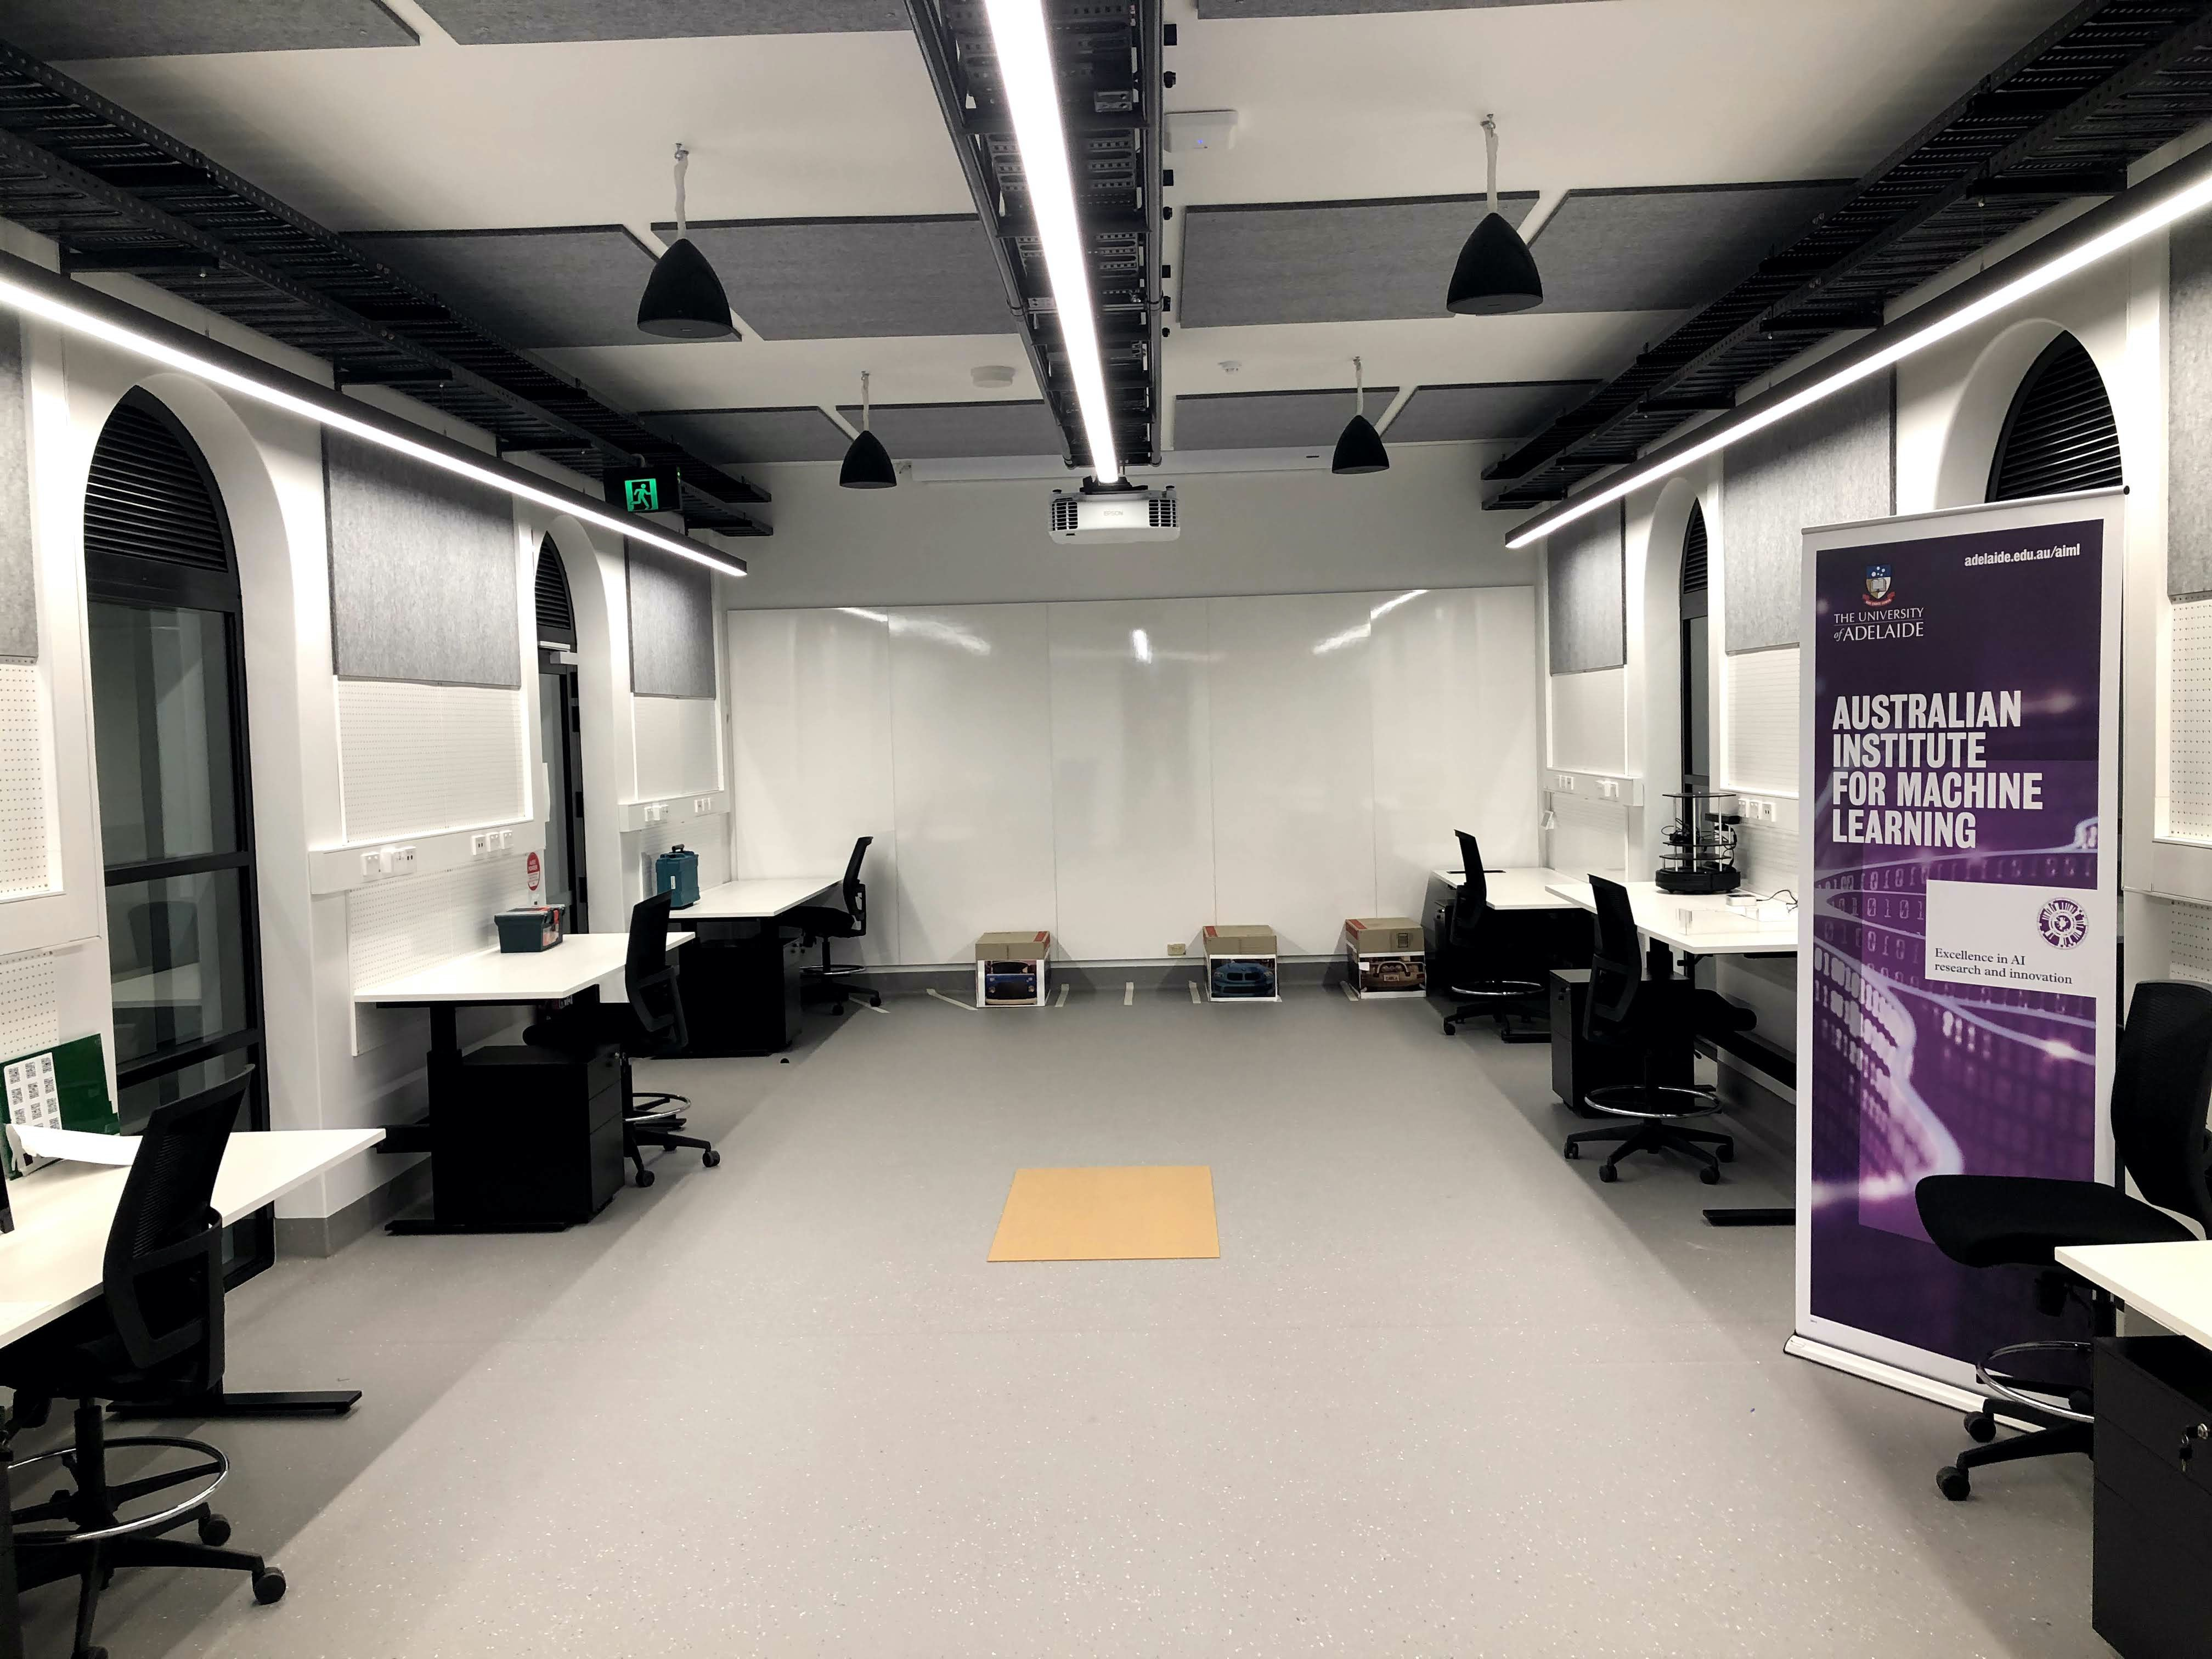
\includegraphics[width=0.95\linewidth]{AutonomousSystems/AIML_edit.jpg}}
  \caption{Raw image 1}
%   \label{fig:cad1}
\end{subfigure}%
\begin{subfigure}[t]{.5\textwidth}
  \centering
  \fbox{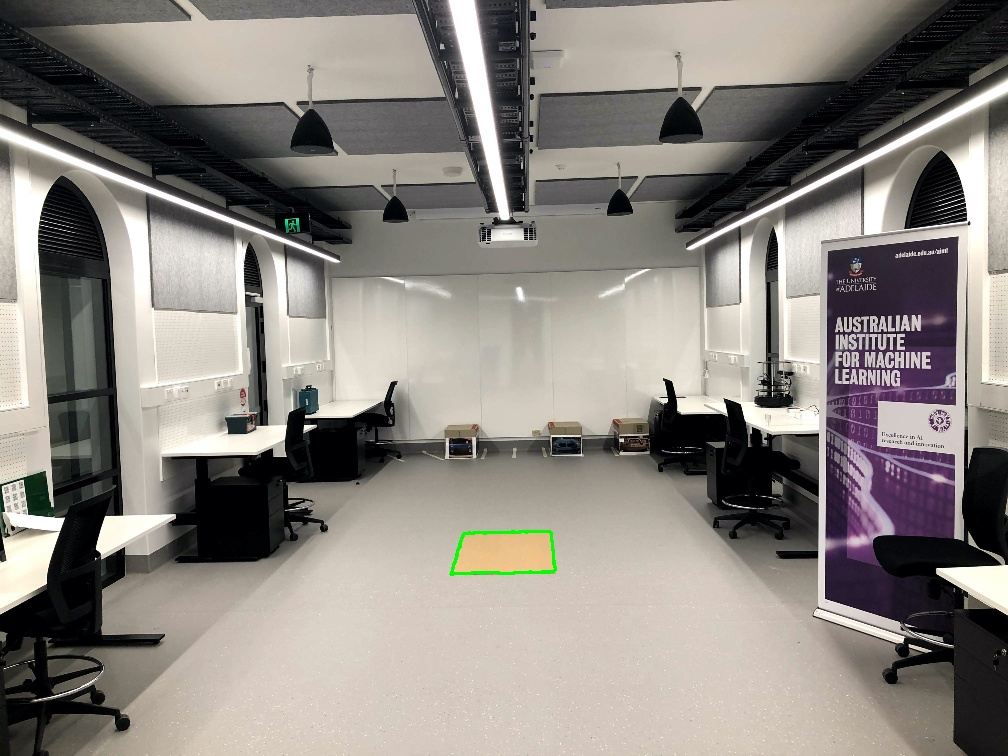
\includegraphics[width=0.95\linewidth]{AutonomousSystems/AIML_edit_ctr.jpg}}
  \caption{Raw image 1 after processing}
%   \label{fig:radar1}
\end{subfigure}
\vskip\baselineskip
\begin{subfigure}[t]{.5\textwidth}
  \centering
  \fbox{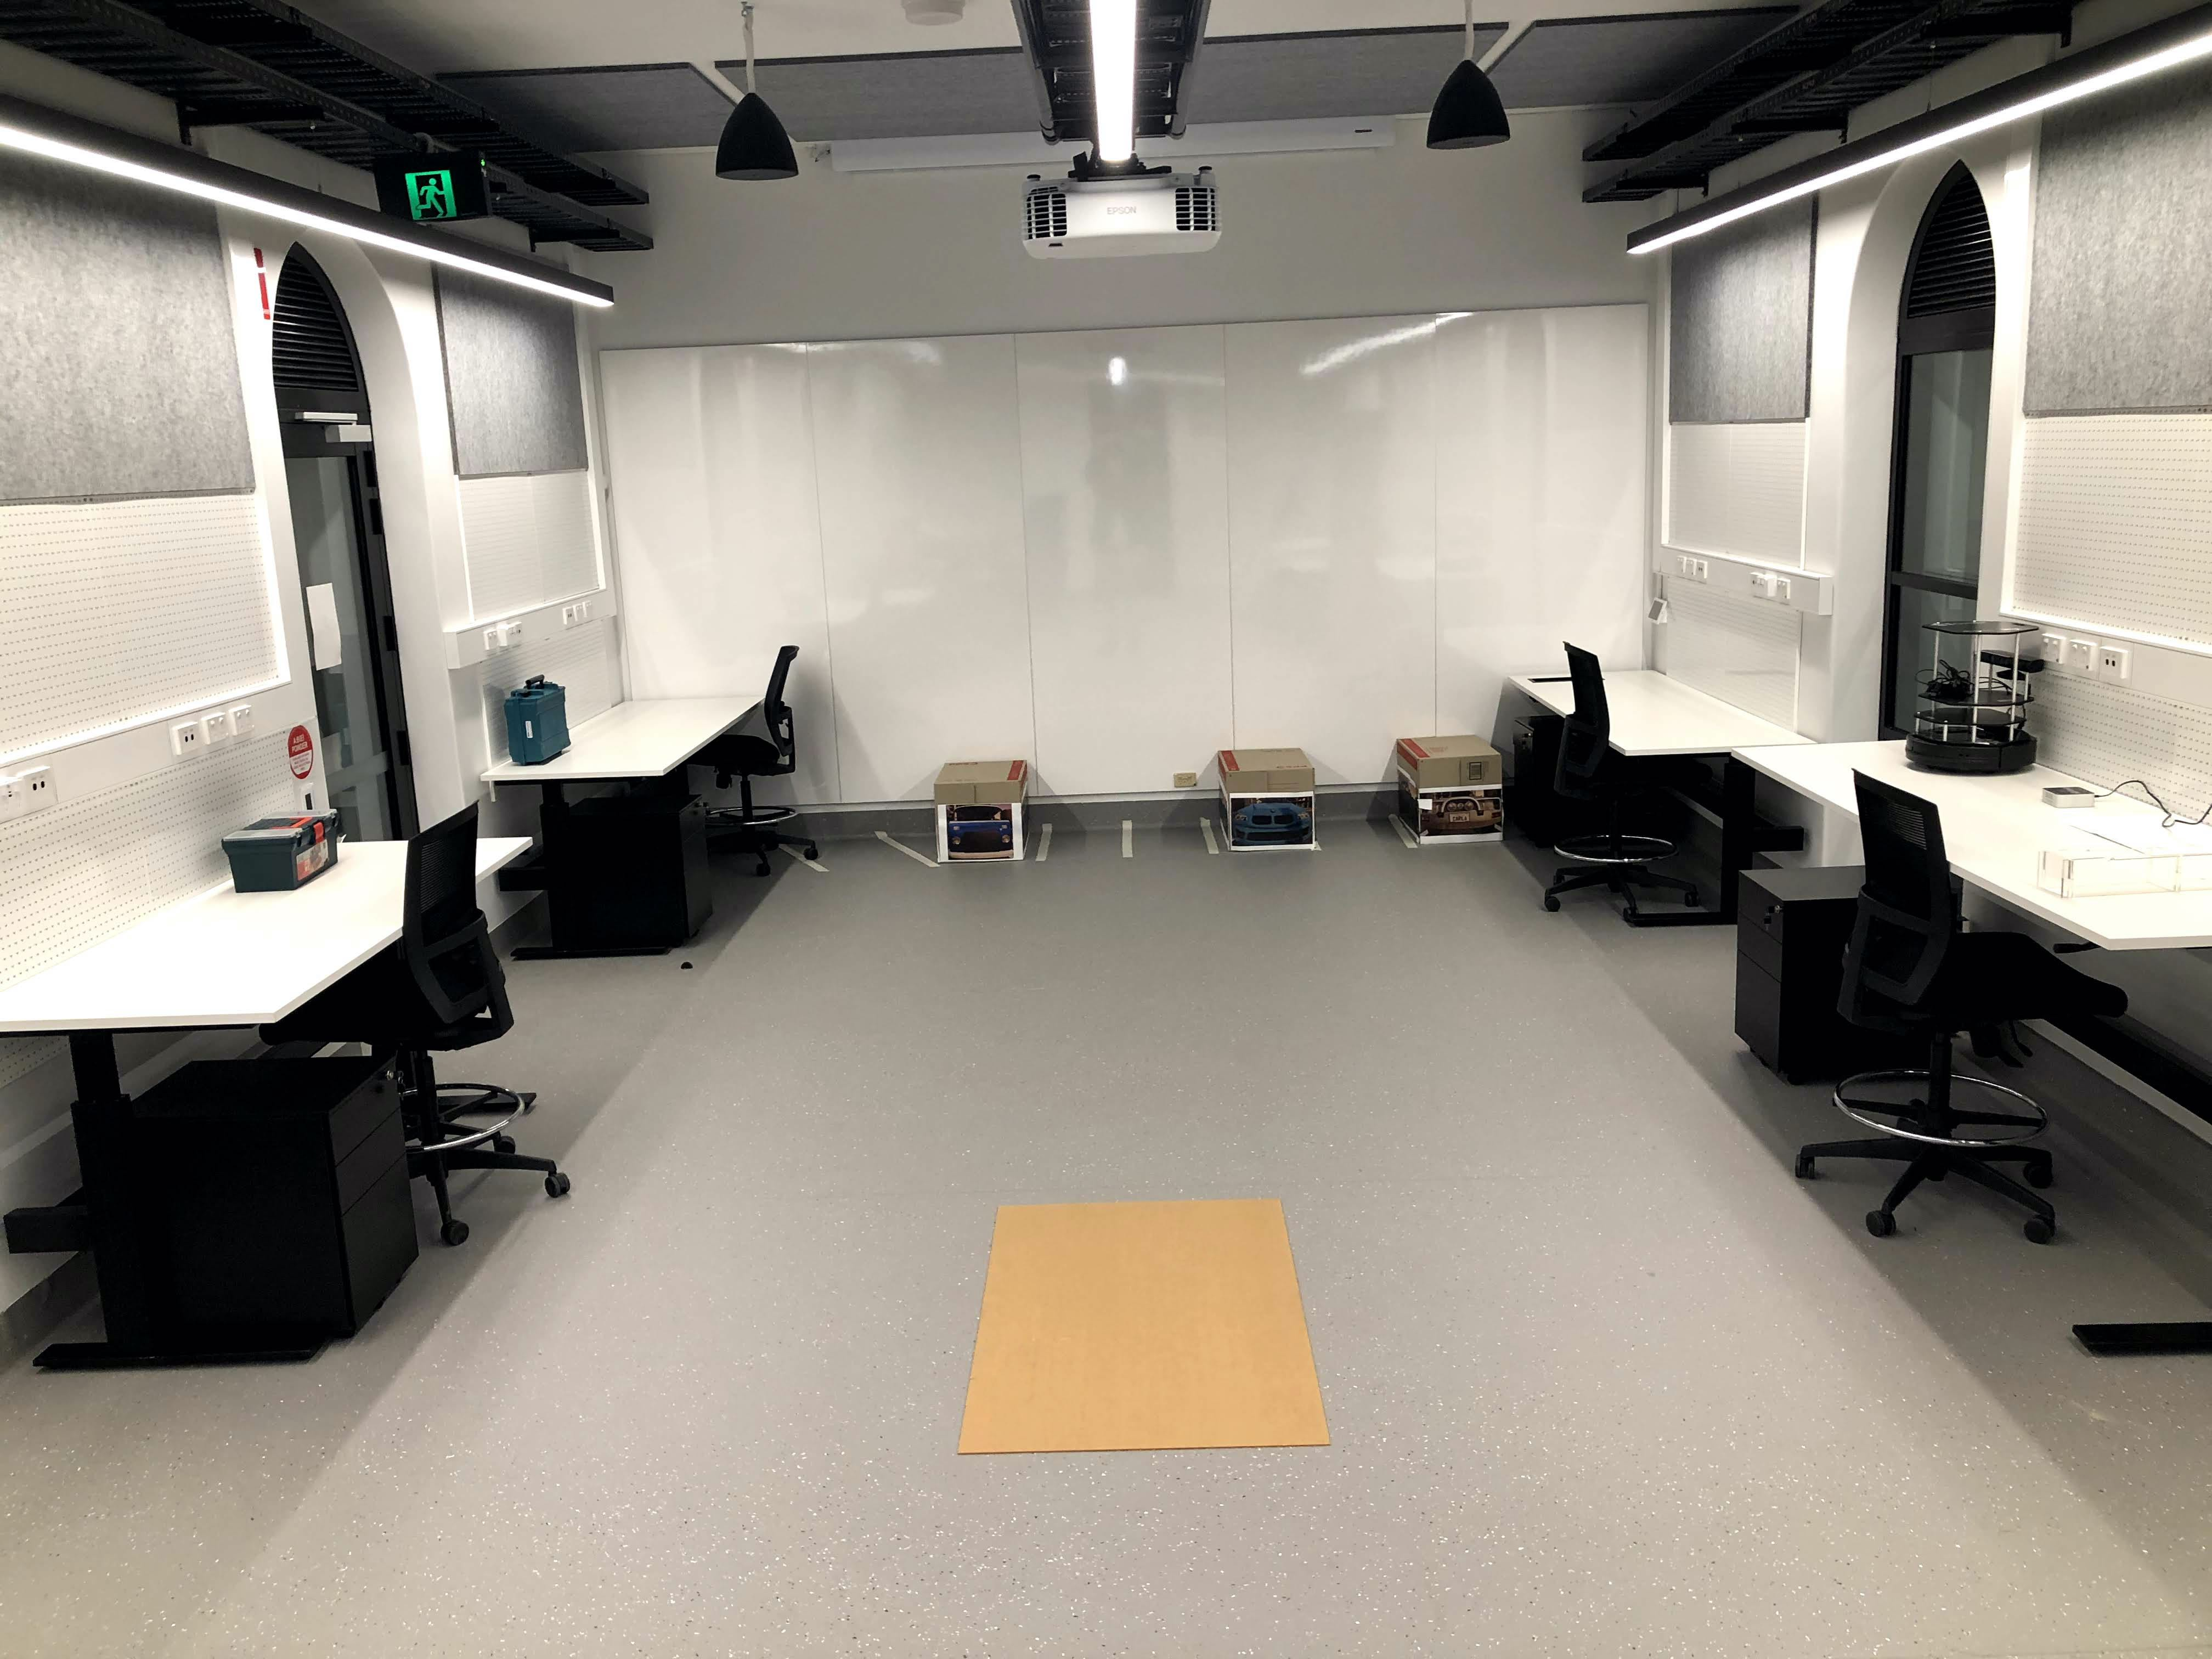
\includegraphics[width=0.95\linewidth]{AutonomousSystems/AIML_edit2.jpg}}
  \caption{Raw image 2}
%   \label{fig:cad1}
\end{subfigure}%
\begin{subfigure}[t]{.5\textwidth}
  \centering
  \fbox{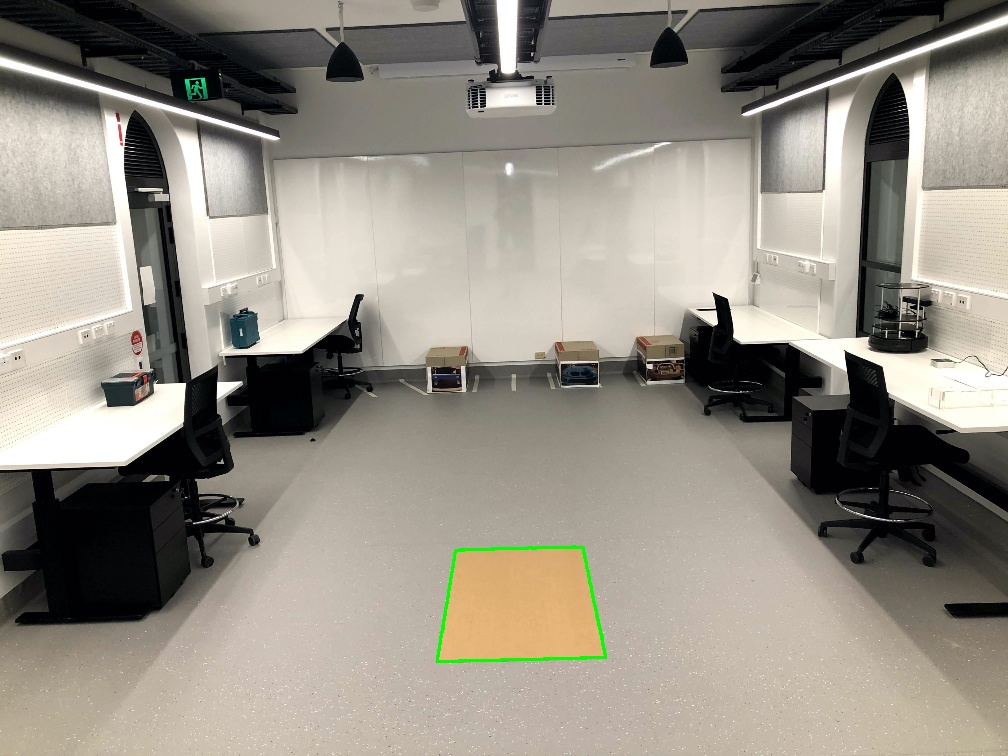
\includegraphics[width=0.95\linewidth]{AutonomousSystems/AIML_edit2_ctr.jpg}}
  \caption{Raw image 2 after processing}
%   \label{fig:radar1}
\end{subfigure}
\caption{Pre- and post-processing images showing landing pad detection.}
\label{fig:landing_detection}
\end{figure}

This was achieved by specifying a colour range that the landing pad fell between, and given the colour was sufficiently distinct from the rest of the space, the system was able to differentiate it from its surroundings. From the mask created by the colour filter, a contour outlining the landing pad was drawn using the \texttt{cv2.findContours()} function. This returned the coordinates of the boundary, which was then coloured green. The code used to implement this is showing in Listing \ref{code}.

\subsubsection{Discussion}
This system worked well in the controlled environment of the laboratory, where it was possible to assume constant lighting colour palette. However, in scenarios more realistic to the application, this method alone is unlikely to be suitable due to variable environmental conditions. The landing pad needs to be more sophisticated in order to differentiate it based on more than just colour as it is unlikely that a single colour will be reliably distinct from its surroundings in all settings.


% \subsubsection{Conclusions}
\subsubsection{Future Work}

Further literature will be reviewed to assess which algorithms are most appropriate for the application, and after testing, the processes will be integrated to form a complete subsystem enabling autonomous landing site detection and descending onboard the UAV. This will be complete and ready to test on the manufactured prototype.